\documentclass[11pt]{article}
\title{How the Codynamic Book Machine Works}
\author{Arthur Petron}
\usepackage[margin=1in]{geometry}
\usepackage{graphicx}
\usepackage{amsmath,amssymb,mathtools}
\usepackage{tikz}
\usetikzlibrary{positioning,arrows.meta}
\usepackage{hyperref}
\graphicspath{{media/}{media/diagrams/}{images/}{artwork/}}

\begin{document}

\section*{Book Repository Layout}

The repository layout is the operational map of the book machine: it separates what the author intends to say from what the system generates, records, and compiles. That separation keeps the project inspectable at every stage, because each class of artifact has a predictable place and a distinct purpose.

At the top level, the repository holds the canonical outline and the working content tree. The outline files describe the book structure, section order, and dependency relationships. The content files hold the prose for each section, usually as source material or normalized section notes before they are rendered into final \LaTeX{}. This division matters because the outline is the control plane, while the section payloads are the writing surface.

Section drafts are stored as \LaTeX{} payloads in per-section files. Each payload corresponds to one section identifier, which makes it possible to regenerate or revise a single section without rewriting the entire book. In practice, this means the authoring system can route work to a section agent, receive a \LaTeX{} body, and write that body to the section payload path associated with the section id. The payloads are therefore the durable draft layer of the repository.

The repository also contains logs and runtime traces. These records capture intake events, normalization steps, agent prompts, task assignments, and revision history. Logs are not part of the prose itself, but they are essential for understanding how a draft came to exist. They provide the audit trail that lets the system explain why a section changed, which agent touched it, and what dependency or blocker shaped the work.

Build artifacts occupy a separate area of the repository. These include compiled outputs, intermediate files, and any generated products created during document assembly. Keeping build artifacts distinct from source content prevents accidental editing of derived files and makes it easier to clean, rebuild, or compare outputs across runs. The source tree remains authoritative, while the build tree remains disposable and reproducible.

Media requests are tracked as first-class artifacts rather than informal notes. When a section needs a figure, diagram, or other visual asset, the request is recorded with enough structure for another agent to fulfill it. The section agent does not invent a file path or silently embed a missing asset; instead, it requests the media through the coordination layer and waits for a returned path and inclusion hint. This keeps visuals synchronized with the text and prevents broken references.

An artifact registry ties these pieces together. It records the generated outputs, their locations, and the relationships among source files, section payloads, media assets, and compiled deliverables. The registry gives the system a single place to answer questions such as which section produced a given \LaTeX{} file, which diagram belongs to which request, or which build artifact corresponds to a particular revision. In that sense, the registry is the repository's index of durable work.

Taken together, the outline files, content sections, \LaTeX{} payloads, logs, build artifacts, media requests, and artifact registry form a layered repository architecture. Each layer has a narrow role, but the layers remain linked through identifiers and recorded events. That structure is what allows the Codynamic Book Machine to treat a book not as a single monolithic file, but as a coordinated set of evolving artifacts.

\begin{figure}[htbp]
\centering
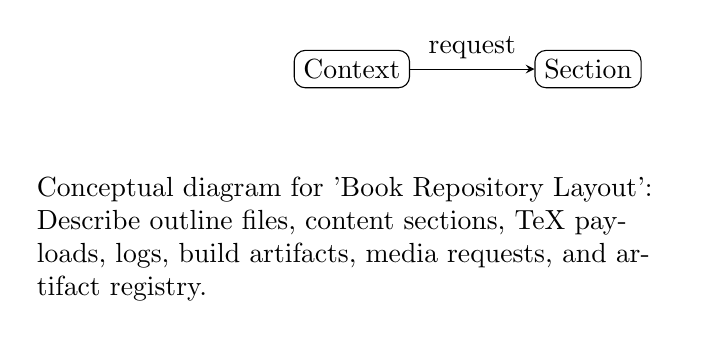
\begin{tikzpicture}[node distance=3cm,>=stealth]
\node[draw, rounded corners] (a) {Context};
\node[draw, rounded corners, right of=a] (b) {Section};
\draw[->] (a) -- node[above] {request} (b);
\node[below=1cm of a, text width=8cm] {Conceptual diagram for 'Book Repository Layout': Describe outline files, content sections, TeX payloads, logs, build artifacts, media requests, and artifact registry.};
\end{tikzpicture}

\caption{Conceptual diagram for 'Book Repository Layout': Describe outline files, content sections, TeX payloads, logs, build artifacts, media requests, and artifact registry.}
\end{figure}


\end{document}
